\documentclass{suturo}

\begin{document}
    \maketitle{Vision}{13.05.2017}{}{1}{}{}{}{}

\makeatletter
\newcommand{\chapterauthor}[1]{%
  {\parindent0pt\vspace*{-47pt}%
  \linespread{2.2}\large\begin{flushright}von: #1\end{flushright}%
  \par\nobreak\vspace*{0pt}}
  \@afterheading%
}
\makeatother

\section*{Architektur und Funktion}
\chapterauthor{Alexander Haar}
Das svm\_classifier-Paket dient zur Ermittlung eines Objektlabels anhand eines Featurevektors.

\subsection{svm\_classifier}
\begin{figure}[!htb]
        \center{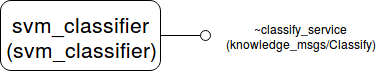
\includegraphics[width= 10cm]
        {figures/svm_classifier.png}
        \caption{\label{fig:classifier} Architektur der storage\_place-node}}
\end{figure}

\subsection{svm\_training\_data\_collector}
\begin{figure}[!htb]
        \center{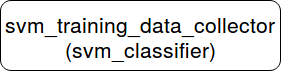
\includegraphics[width= 5cm]
        {figures/svm_training_data_collector.png}
        \caption{\label{fig:training_data} Architektur der storage\_place-node}}
\end{figure}

\subsection{svm\_trainer}
\begin{figure}[!htb]
        \center{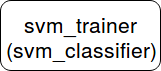
\includegraphics[width=5cm]
        {figures/svm_trainer.png}
        \caption{\label{fig:trainer} Architektur der storage\_place-node}}
\end{figure}
      
\section*{Methodendokumentation}
\chapterauthor{Alexander Haar}
\subsection{svm\_classifier}
\subsubsection{main - Python}
\begin{verbatim}
if __name__ == '__main__'
Beschreibung: Lädt die svm_model.sav Datei und startet den Classify- Service.
\end{verbatim}
\subsection{svm\_training\_data\_collector}

\subsubsection{save\_training\_set - Python}
\begin{verbatim}
def save_training_set()
Beschreibung: Nachdem alle Trainingsdaten gesammelt wurden, speichert diese 
Funktion alle Daten als sav- Datei.
\end{verbatim}

\subsubsection{get\_corresponding\_normals\_histogram\_file - Python}
\begin{verbatim}
def get_corresponding_normals_histogram_file(color_histogram_file)
Beschreibung: Findet zu einem Farbhistogramm das entsprechende Normalshistogramm. 
@param color_histogram_file: Das Farbhistogramm.
@return: Das korrespondierende Normalshistogramm.
\end{verbatim}

\subsubsection{get\_features - Python}
\begin{verbatim}
def get_features(label, color_histogram_file)
Beschreibung: Ermittelt anhand des Labels der Klasse und der Farbhistogrammdatei 
den Featurevektor
@param label: Das Label der Klasse.
@param color_histogram_file: Die Farbhistogrammdatei.
@return: Der resultierende Featurevektor.
\end{verbatim}

\subsubsection{collect\_training\_data - Python}
\begin{verbatim}
def collect_training_data()
Beschreibung: Startet das Sammeln von Trainingsdaten.
\end{verbatim}

\subsubsection{main - Python}
\begin{verbatim}
if __name__ == '__main__'
Beschreibung: Initialisiert den Paketpfad und startet das Sammeln 
von Trainingsdaten.
\end{verbatim}

\subsection{svm\_trainer}

\subsubsection{plot\_confusion\_matrix - Python}
\begin{verbatim}
def plot_confusion_matrix(cm, classes, normalize=False, title='Confusion matrix',
cmap=plt.cm.Blues)
Beschreibung: Erstellt eine Konfusionsmatrix und stellt diese graphisch dar. 
@param cm: Die echten Labels.
@param classes: Die vorhergesagten Labels.
\end{verbatim}

\subsubsection{main - Python}
\begin{verbatim}
if __name__ == '__main__'
Beschreibung: Lädt die Trainingsdaten und startet das Trainieren der SVM, 
welche anschließend gespeichert wird.
\end{verbatim}

\section*{Schnittstellen}
\chapterauthor{Alexander Haar}

\subsection*{Service Server classify\_service}
\begin{verbatim}
def classify(req)
Beschreibung: Service- Methode, welche einen Featurevektor klassifiziert.
@param req: Die Anfrage an den Service, welche den Featurevektor enhält.  
@param res: Die Antwort des Services, welche das Label enthält.
\end{verbatim}

\section*{Programmablauf}
\chapterauthor{Alexander Haar}
\subsection*{Schritt 1: Trainingsdaten sammeln und speichern}
Es werden aus csv- Dateien die Featurevektoren mit Labels ausgelesen und als sav- Datei gespeichert.

\subsection*{Schritt 2: Trainieren und speichern einer SVM} 
Die Trainingsdaten werden geladen, danach wird eine SVM mit den Daten trainiert und gespeichert.

\subsection*{Schritt 3: Laden der SVM und Klassifizieren von Featurevektoren}
Die beiden vorherigen Schritte werden nur einmal im Vorfeld ausgeführt. Das Hauptprogramm lädt die SVM und startet anschließend den Classify- Service.

\end{document}
